\subsection{Hydrostatic Force}

Hydrostatic force is the force an object feels when it's submerged by a liquid. It's defined 
by the liquid's density, surface area of the object, and the acceleration felt by gravity. The force changes since different parts of the object is submerged at different heights. 

\begin{equation}
	F = \delta dgA
\end{equation}

Do note, that this formula only works with horizontal strips as vertical plates will have different pressures at different depths.  

\paragraph*{Let's do an example problem}. Consider a triangle who's base is 6 meters long and it's right on the water's surface. The triangle's height is 4 meters. The force is going to be applied down on the triangle, so if we use a vertical x-axis, where $x=0$ is the surface of the water, and $x=4$ is the depth at which the tip of the triangle is, we can defined our horizontal strips has $\Delta x$. The black strip in the image is a good repersentation of what we are going for.

\begin{figure}[H]
	\begin{center}
		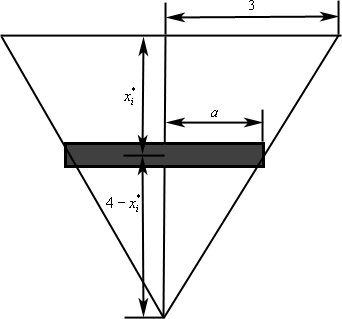
\includegraphics[scale=0.45]{pages/images/hystatic}
		\caption{from: tutorial.math.lamar.edu/Classes/CalcII/HydrostaticPressure.aspx}	
		\label{fig:test_figure}
	\end{center}
\end{figure}

Now for our area function, we can find the width of the triangle at different x distances, by using similar triangles.

\begin{align*}
	\frac{3}{4} &= \frac{a}{4-x_i} \\ 
	2a &= \frac{3(4-x_i)}{2}
\end{align*}

Now since this is going to add all the strips together, we don't need to do our area of a triangle equation. 

\begin{align}
	A &= 2a\Delta x 
\end{align} 
\begin{align}
	F = \delta dgA \to F = \delta g \int_0^42a(x)dx \to F = \delta g\int_0^4\frac{3x(4-x)}{2}dx
\end{align}
